\documentclass{IMEKO2024}

%%%% Packages %%%%%%%%%%%%%%%%%%%%%%%%%%%%%%%%%%%%%%%%%%%%
\usepackage{amsmath}
\usepackage[colorlinks=true]{hyperref}
\usepackage{microtype}
\usepackage{proof}
\usepackage{mathtools}
\usepackage{graphicx}
\usepackage{rotating}
\usepackage{subcaption}
%\usepackage{multirow}
\usepackage{xkeyval}
\usepackage[font=small,justification=centering]{caption}
\captionsetup{labelsep = period}
\usepackage{subcaption}
\usepackage{floatrow}

%%%%%%%%%%%%%%%%%%%%%%%%%%%%%%%%%%%%%%%%%%%%%%%%%%%%%%%%%%

%%%% Macros %%%%%%%%%%%%%%%%%%%%%%%%%%%%%%%%%%%%%%%%%%%%%%
\newcommand{\pct}{\texttt{\symbol{37}}}
\newcommand{\dir}{\texttt{\symbol{62}}}
\newcommand{\res}{\texttt{\symbol{60}}}
\newcommand{\lcb}{\texttt{\symbol{123}}}
\newcommand{\rcb}{\texttt{\symbol{125}}}
\newcommand{\lsb}{\texttt{\symbol{91}}}
\newcommand{\bsl}{\texttt{\symbol{92}}}
\newcommand{\rsb}{\texttt{\symbol{93}}}

\newcommand{\istype}[1]{#1\ \textsf{type}}
\newcommand{\isadd}[1]{#1\ \textsf{numeric}}
\newcommand{\ismult}[3]{(#1, #2, #3)\ \textsf{multipliable}}

\newcommand{\append}{\mathop{+\!\!+}}
\newcommand{\hjux}[2]{{#1}|{#2}}
\newcommand{\vjux}[2]{\frac{#1}{#2}}

\newcommand{\One}{\mathbf{1}}
\newcommand{\Matrix}[5]{\mathsf{Matrix}\,#1\,#2\,#3\,#4\,#5}
\newcommand{\List}[1]{\mathsf{List}\,#1}

\newcommand{\remph}{\emph}

\newcommand{\todo}[1]{\textcolor{red}{\textbf{TODO: #1}}}

\newcommand{\param}{parametrize}
%%%%%%%%%%%%%%%%%%%%%%%%%%%%%%%%%%%%%%%%%%%%%%%%%%%%%%%%%%

\begin{document}

\title{LabMate: a prospectus for types for MATLAB}
\author{Conor McBride  \affiliationmark{1}, Georgi Nakov  \affiliationmark{1}, Fredrik Nordvall Forsberg  \affiliationmark{1}, Andr\'e Videla  \affiliationmark{1}, Alistair Forbes  \affiliationmark{2}, Keith Lines  \affiliationmark{2}}
\affiliation{%
\affiliationmark{1}{\fontsize{11pt}{9pt} \selectfont University of Strathclyde , UK}  \\
\affiliationmark{2}{\fontsize{11pt}{9pt} \selectfont National Physical Laboratory, UK}}

\maketitle

\begin{abstract}
  Many computations in science and engineering are implemented in the
  programming language MATLAB. However the high-level meaning of such
  MATLAB programs stay informal, which can lead to implementation
  errors and bugs, for example relating to incompatible units of
  measure for quantities, or incompatible sizes of matrices at
  runtime. We are in the process of developing LabMate, which is a
  tool for reifying current informal programmer practices into a
  language of formal comments. These comments are ignored by MATLAB,
  but acted on and checked by LabMate. We outline the design
  principles behind LabMate, our current progress, and our future
  plans.
\end{abstract}

\begin{keywords}
  MATLAB, software correctness, dimensional consistency, type theory
\end{keywords}

\section{Introduction}

MATLAB is a key workhorse in many scientific and engineering
disciplines that are heavily reliant on numerical methods. It helps us
do powerful things. However, as with all software, MATLAB code may
contain implementation errors and bugs. In good programming practice
for MATLAB developers, programmers use comments to make clear what
physical systems their data concern and how the data should be
interpreted, specifying, e.g., units of measure for
quantities. Regrettably, none of this rich and often disciplined
metadata is perceptible to MATLAB, which instead enforces the
compatibility of producers and consumers of data by run-time checking
of tags which indicate only machine representation, not any form of
meaning. In reality, the programmers document meaning for each other's
benefit but keep the machine in the dark.

To rectify this situation, we have developed LabMate, which is a tool
to reify current virtuous engineering practices as a formal language
of MATLAB comments. MATLAB remains in the dark, but LabMate reads,
assesses, and transforms MATLAB programs in accordance with these
comments.
%
Behind the scenes, LabMate is retrofitting an expressive type system
to MATLAB, with the more of the meaning of programs recorded in their
types.
%
This gives a lightweight and low-cost way for MATLAB programmers to
express their intent, and in a language they are already working in,
rather than starting over from scratch.
%
While type systems and their theory is a well established discipline
of computer science, the development of LabMate has several novel
advances on the algebraic structure required to classify
matrices and the meanings of the quantities therein, e.g., their
physical dimensions. LabMate brings advanced type systems to
effectiveness within, rather than instead of, existing scientific and
engineering toolchains and practices.

LabMate is under constant development; the latest version can be found at \url{https://github.com/msp-strath/LabMate/tree/devel}.
%
At time of writing, the necessary core type system is in place: we are busily extending the variety of MATLAB expressions it can make sense of, and the constraints it can solve.
%
We are close to covering the examples in this paper, but not quite there yet.
%
We aim to eliminate the speculative future tense from our examples before camera-ready copy is required.
%
This paper effectively documents how far we have come, and the roadmap to our next milestone.

\section{LabMate in action}
\label{sec:example}

% simple matrix multiplication example

The following greatly simplified, but still realistic, example from metrology  will help illustrate the principles of how LabMate will work. Consider one of the calculations required for measuring resistors using a cryogenic current comparator bridge~\cite{Williams_2010}.

An electrical current with a known value (the applied signal) is passed through the resistor being measured, and a series of voltage readings are taken at fixed time intervals (the recorded output). After a specified number of readings are taken, the direction of the input signal must be reversed in order to separate the offset and drift from the voltage readings. Therefore, the applied signal (bridge energisation) is a square wave of {\em reversals}. A calibration factor is also applied, dividing the signal into two parts with different amplitudes.

The recorded output follows the input signal, superimposed on a detector with noise, offset and drift. Figure~1%\ref{fig:rec_out}
provides an example of recorded output, using simulated data.
\begin{figure}[H]
  \begin{center}
    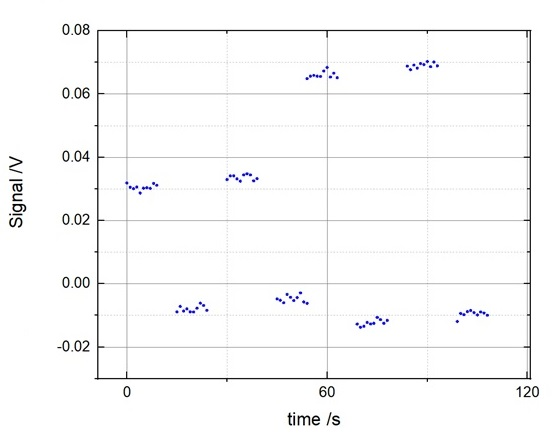
\includegraphics[width=0.6\linewidth]{example_output.jpg}
    \captionwide{Simulated example of recorded output.}
    \label{fig:rec_out}
  \end{center}
\end{figure}

The calculation of offset and drift is achieved using a least squares line fit calculated by solving a series of simultaneous equations, listed below. Note that although offset and drift differ for calibration and non-calibration parts of the input signal, the drift is the same in both cases.

% $t_i$ time ($\mathsf{T}$; in seconds); $v_i$ voltage ($\mathsf{ML}^2\mathsf{T}^{-3}\mathsf{I}^{-1}$; in volt)

\[
\begin{pmatrix*}
  d_{\textrm{nc}1} & d_{\textrm{c}1} & n_1 & c_1 & t_1  \\
  d_{\textrm{nc}2} & d_{\textrm{c}2} & n_2 & c_2 & t_2  \\
   & \vdots &  & & \\
  d_{\textrm{nc}N} & d_{\textrm{c}N} & n_N & c_N & t_N  \\
\end{pmatrix*}
\times
\begin{pmatrix}
  a \\
  a_{cal} \\
  c \\
  c_{cal} \\
  m
\end{pmatrix}
=
\begin{pmatrix}
  v_1 \\
  v_2 \\
  \vdots \\
  v_N
\end{pmatrix}
\]
%
The matrix left of $\times$ is made up of the following values:
%
\begin{itemize}
    \item The values in the first four columns are purely numeric and have no associated dimension.

    \item The first column will contain either $1$ or $-1$ for non-calibration voltage readings (i.e., those to which the calibration factor has not been applied) depending on the direction of the input signal. For calibration readings the value will be $0$.

    \item The second column contains equivalent values for voltage readings in which the calibration factor has been applied, i.e., $0$ for non-calibration readings and $1$ or $-1$ depending on the input signal direction for calibration readings.

    \item The third column contains $1$ for non-calibration readings and $0$ for calibration.

    \item The fourth column is the opposite of the third.

    \item The fifth column contains time values.
\end{itemize}

The column vector right of $\times$ and left of $=$ contains values to
be calculated using the line fit which then determine the measured
value of the resistor by a calculation which is beyond the scope of
this paper. The column vector right of $=$ contains voltage readings.

This calculation can be converted into a MATLAB problem using the
builtin left division operator {\bsl} to compute a
least squares fit. Let us step through how we intend to use LabMate to
help us deliver this solution.

We begin by declaring the types of the input data: the \texttt{times} and the \texttt{voltages}. Our example calculation uses twelve time and voltage inputs, arranged as two rows to be read from a file. A real measurement would involve considerably larger datasets.
\begin{verbatim}
%> times    :: [ 1 x 12 ] double
%> voltages :: [ 1 x 12 ] double
\end{verbatim}
Lines starting with `\texttt{\%>}' are interpreted as ordinary comments by MATLAB, but as \remph{directives} by LabMate, here giving us enough information not only to insist that the values of \texttt{times} and \texttt{voltages} \remph{conform} to the given sizes, but to determine \remph{how} to read them from a file. We would issue the further directive
\begin{verbatim}
%> readfrom "inputs.txt" times voltages
\end{verbatim}
LabMate is a program \remph{transducer}: its output is a modified version of its input, allowing it to respond to directives with information in comments or by generating code. Here we would expect to see something like
\begin{verbatim}
%> readfrom "inputs.txt" times voltages
%<{
h=fopen("inputs.txt");
c=textscan(h,'%f');
fclose(h);
src = c{1};
readPtr = 1;
for i = 1:12
  times[i] = src[readPtr];
  readPtr = readPtr + 1;
end
for i = 1:12
  voltages[i] = src[readPtr];
  readPtr = readPtr + 1;
end
%<}
\end{verbatim}
where the comment lines `\pct\res\lcb' and `\pct\res\rcb' visually delimit the extent of the generated boilerplate code, so that humans may safely ignore it. LabMate knows enough about scope in MATLAB to ensure that auxiliary variable naming never creates conflict. We have kept to one datum per line for simplicity, but we are free to extend our format specification language as we see fit~\cite{mgen}.

Next, let us build up the matrix in the calculation. The method gives the first four columns a pattern of blocks, pasted in a grid.
\begin{verbatim}
%> z3 :: [ 3 x 1 ] double
z3 = [ 0; 0; 0 ]
%> i3 :: [ 3 x 1 ] double
i3 = [ 1; 1; 1 ]

ddnc = [ i3  z3  i3  z3
        -i3  z3  i3  z3
         z3  i3  z3  i3
         z3 -i3  z3  i3 ]
\end{verbatim}
LabMate will check that this pasting strategy delivers a rectangular matrix, well in advance of MATLAB runtime. Pasting on the measured times (transposed to a column) completes the matrix. Let us ask for its type. LabMate responds to information-seeking directives by writing comments of its own, beginning with `\pct\res'.
\begin{verbatim}
M = [ ddnc times' ]
%> typeof M
%< M :: [ 12 x 5 ] double
\end{verbatim}

Now that we have assembled the data, we may solve the equations and ask for the type of the solution.
\begin{verbatim}
x = M \ voltages
%> typeof x
\end{verbatim}
Did you notice the error in the above code? The vector \texttt{voltages} should be of size $12 \times 1$, but is erroneously of size $1 \times 12$ instead. LabMate detects this error and responds:

\begin{verbatim}
x = M \ voltages
%< unsolved constraint 12 =? 1
%> typeof x
%< the type of x is quite a puzzle
\end{verbatim}
%
That is, LabMate says that for \texttt{x} to have a sensible type, we need \texttt{M} and \texttt{voltages} to have the same number of rows. We forgot to transpose \texttt{voltages}! If we make the necessary repair, we should now see something more satisfying.
\begin{verbatim}
x = M \ voltages'
%> typeof x
%< x :: [ 5 x 1 ] double
\end{verbatim}
This way, LabMate can detect matrix size errors at development time, rather than at runtime --- running the original code would indeed crash with the error:
\[\textcolor{red}{\textbf{\texttt{Matrix dimensions must agree}}}\]

\section{Types for matrices}

\newcommand{\rs}{\mathit{rs}}
\newcommand{\ms}{\mathit{ms}}
\newcommand{\cs}{\mathit{cs}}

Under the hood, LabMate translates selected well behaved MATLAB expressions
to typed expressions in its own core theory of types and values.
%
As matrices feature heavily in MATLAB code, the types of matrices
play a central role in this theory.
%
In particular, we acknowledge that the rows and columns of a matrix might pertain to distinct individual entities, rather as the rows ans columns of a spreadsheet do.
%
Internally, a matrix type looks like
\[\Matrix{R}{C}{E}{\rs}{\cs}
\]
%
We thus \param{} matrix types by two arbitrary `header' types $R$, for the individuals the rows concern, and $C$ for the columns. We may then give two lists, $\rs = [r_1,\ldots,r_m]\in\List{R}$ (so that each $r_i\in R$) and $\cs = [c_1,\ldots,c_n]\in\List{C}$ of those individuals. A \param{}d type $E(r,c)$ gives the type of entry for any combination of row and column individual, with $E(r_i,c_j)$ being the type of the entry $e_{i,j}$. In the diagram below, the $e$s inside the rectangle are the matrix entries computed by the MATLAB code. The $r$s and $c$s outside the rectangle are \remph{meta}data coming from the matrix type, known only to LabMate, and not available as data to MATLAB.
\[\begin{array}{@{}r|ccccc|}
\; & c_1      & \cdots & c_j     & \cdots & c_n     \\
\hline
r_1    & e_{1,1}  &        & e_{1,j} &        & e_{1,n} \\
\vdots &          &        &         &        &         \\
r_i    & e_{i,1}  &        & e_{i,j} &        & e_{i,n} \\
\vdots &          &        &         &        &         \\
r_m    & e_{m,1}  &        & e_{m,j} &        & e_{m,n}  \\
\hline
\end{array}\]
To check that $\Matrix{R}{C}{E}{\rs}{\cs}$ is a valid type, LabMate must:
\begin{enumerate}
\item check that $R$ and $C$ are both valid types;
\item check that $E(r,c)$ is a valid type whenever $r\in R$ and $c\in C$;
\item check that $\rs\in\List{R}$ and $\cs\in\List{C}$.
\end{enumerate}

A notable special case is when both $R$ and $C$ are the unit type $R = C = \One$, that is, the type with exactly one element.
%
$\List{\One}$ amounts to a mere `tally', counting indistinct things, which we allow to be written as a number in decimal notation.
%
In this case, there is only one type of entries $E(r,c)$ (because both $r$
and $c$ must be the unique element of the unit type), and the only
information available in the lists $\rs : \List{\One}$ and
$\cs : \List{\One}$ are their lengths.
%
Thus, we have recovered $\Matrix{\One}{\One}{E}{m}{n}$ as the type of
$m \times n$ matrices with entries of type $E$, where $m$ and $n$ are
the unique lists over the unit type of length $m$ and $n$
respectively.
%
That is what we render in LabMate directives and responses as
\[
\lsb \;m \;\texttt{x}\; n\; \rsb\; E
\]
as in our \texttt{M :: [ 1 x 5 ] double} in Section~\ref{sec:example}.

So much for what it is to be a valid matrix type: what does it mean to be a valid matrix \remph{in} such a type?

Firstly, a singleton entry matrix must have singleton header lists $[r]$ and $[c]$.
\[\begin{array}[b]{@{}r|@{}c@{}|l}
\; & c \\
\cline{1-2}
r  & e\in E(r,c) & \quad \in \Matrix{R}{C}{E}{[r]}{[c]} \\
\cline{1-2}
\end{array} 
\]

Secondly, to check a horizontal pasting of matrices, we must ensure that the header and entry types match, that the row headers are the same for left and right, and that the column headers can be split into a prefix for the left matrix and a suffix for the right. In other words, the column headers for the whole are the concatenation ($\append$) of the column headers for the parts.
\[\begin{array}{l}
\begin{array}{@{}r|c|c|}
  & \cs_A & \cs_b \\
\hline
&&\\
&A \in & B \in \\
\rs &\Matrix{R}{C}{E}{\rs}{\cs_A} & \Matrix{R}{C}{E}{\rs}{\cs_B} \\
&&\\
\hline
\end{array}\bigskip\\
\;\;\; \in \Matrix{R}{C}{E}{\rs}{(\cs_A\append\cs_B)}
\end{array}\]

Thirdly, vertical pasting is similar, except that it is the row headers which split into prefix and suffix while the column headers are shared.
\[
\begin{array}[c]{@{}r|c|}
  & \cs \\
  \hline
  \;    & \\
  \;    & A \in \\
  \rs_A & \Matrix{R}{C}{E}{\rs_A}{\cs} \\
  \;    & \\
  \hline
  \;    & \\
  \;    & B \in \\
  \rs_B & \Matrix{R}{C}{E}{\rs_B}{\cs} \\
  \;    & \\
  \hline
\end{array}
\in
\begin{array}{l}
\Matrix{R}{C}{E}{\\ \quad (\rs_A\append\rs_B)}{\cs}
\end{array}
\]

Now that we have matrices, we must explain how to typecheck matrix operations.

To check if we may add matrices $A$ and $B$, LabMate must:
\begin{enumerate}
\item check that $A$ and $B$ both have the \remph{same} matrix type $\Matrix{R}{C}{E}{\rs}{\cs}$;
\item check that \remph{every} entry type $E(r,c)$ admits addition.
\end{enumerate}
In the short term, LabMate can get by with a hard-coded table of which types (e.g. \texttt{double}) admit addition, but more flexible and general approaches to operator overloading (e.g., Haskell's `type classes'~\cite{wadler.blott}) are readily adoptable in due course.

Multplication is rather more involved, of course. The usual requirement that the matrix sizes `meet in the middle' generalises straightforwardly to lists of headers,
\[\begin{array}{@{}c@{}}
\begin{array}[c]{@{}r|c|}
  \;  & \ms \\
  \hline
  \;  &     \\
  \;  &  A \in \\
  \rs & \Matrix{R}{M}{E_1}{\rs}{\ms} \\
  \;  & \\
  \hline
\end{array}
  \times
\begin{array}[c]{@{}r|c|}
  \;  & \cs \\
  \hline
  \;  &     \\
  \;  &     \\
  \;  &  B \in \\
  \ms & \Matrix{M}{C}{E_2}{\\ & \ms}{\cs} \\
  \;  &     \\
  \;  & \\
  \hline
\end{array}
\bigskip\\
\in \qquad
\begin{array}[c]{@{}r|c|}
  \;  & \cs \\
  \hline
  \;  &     \\
  \rs & \Matrix{R}{C}{E_3}{\\ & \rs}{\cs} \\
  \;  & \\
  \hline
\end{array}
\end{array}
\]
but we must also check that the entry types are compatible. Specifically, LabMate must:
\begin{enumerate}
  \item check, for all $r$, $m$ and $c$, that if $a\in E_1(r,m)$ and $b\in E_2(m,c)$, then
    $a\times b \in E_3(r,c)$;
  \item check that \remph{every} entry type $E_3(r,c)$ admits addition.
\end{enumerate}

These conditions are straightforward in the special case where $R = C = \One$ and the $E$s are standard numerical types. There are, however, more motivating possibilities.

Of particular interest is the case when the header types, $R$ and
$C$, are types of physical dimensions, with $E(r, c)$ being the
type of physical quantities of dimension $r^{-1}\cdot c$.
%
Such quantities admit addition only if the dimensions match. Meanwhile, their multiplication correspondingly multiplies the dimensions.
%
This way, we can reduce dimensional consistency checking \`a la
Kennedy~\cite{kennedyUOM} to typechecking, but also for programs involving matrices of non-uniform dimension, following the work of Hart~\cite{hart}.
%
We will see in Section~\ref{sec:example-revisited} how this can be helpful.


%Matrix types formation can thus be summarised as the inference rule given in Figure~\ref{fig:matrix_intro}.
%\[
%  \infer{\istype{\Matrix{R}{C}{E}{rs}{\cs}}}
%  {
%    \istype{R}
%    &\quad
%    \istype{C}
%    &\quad
%    x : R, y : C \vdash \istype{E(x,y)}
%    &\quad
%    rs : \List{R}
%    &\quad
%    cs : \List{C}
%  }
%\]
%
%\begin{figure*}[th]
%\begin{subfigure}{\textwidth}
%  \begin{center}
%    \[
%      \infer{\istype{\Matrix{R}{C}{E}{\rs}{\cs}}}
%      {
%        \istype{R}
%        &\quad
%        \istype{C}
%        &\quad
%        x : R, y : C \vdash \istype{E(x,y)}
%        &\quad
%        \rs : \List{R}
%        &\quad
%        \cs : \List{C}
%      }
%    \]
%  \end{center}
%  \caption{Type formation rule for matrix types}
%  \label{fig:matrix_intro}
%\end{subfigure}
%\hfill
%\begin{subfigure}{\textwidth}
%  \begin{center}
%    \[
%      \infer{A + B : \Matrix{R}{C}{E}{\rs}{\cs}}
%      {
%        x : R, y : C \vdash \isadd{E(x, y)}
%        &\quad
%        A : \Matrix{R}{C}{E}{\rs}{\cs}
%        &\quad
%        B : \Matrix{R}{C}{E}{\rs}{\cs}
%      }
%    \]
%  \end{center}
%  \caption{Addition rule for matrices}
%  \label{fig:matrix_add}
%\end{subfigure}
%\hfill
%\begin{subfigure}{\textwidth}
%  \begin{center}
%    \[
%      \infer{A * B : \Matrix{R}{C}{E''}{\rs}{\cs}}
%      {
%        \ismult{E}{E'}{E''}
%        &\quad
%        A : \Matrix{R}{C}{E}{\rs}{\ms}
%        &\quad
%        B : \Matrix{R}{C}{E'}{\ms}{\cs}
%      }
%    \]
%  \end{center}
%  \caption{Multiplication rule for matrices}
%  \label{fig:matrix_mul}
%\end{subfigure}
%% FIXME : \caption is broken
%\captionwide{Typing rules for matrices}
%\label{fig:matrix_rules}
%\end{figure*}

Checking the compatibility between operations and data boils down to checking equality of types. LabMate types are \remph{dependent} types, in the style of the state-of-the-art functional programming languages Agda and Idris~\cite{ydtm,agdathing,idristhing}. Dependent types express the reality that data validity is often a \remph{relative} notion, with the compatibility requirements for matrix multiplication being a standard example. Types which mention (hence depend on) some values (e.g., our header lists) are used to classify other values (e.g., our matrices) with respect to them.

Equality of types therefore demands some notion of equality for the values they mention. We equip every type in our core theory with an algorithmic decision procedure testing when two expressions in the type are sufficiently obviously equal to guarantee compatibility of types. Languages like Agda and Idris generate their notion of expression equality by extending the evaluation rules used to compute with values at runtime to cope with expressions involving variables by getting stuck whenever a variable prevents a condition from being tested. In MATLAB, the matrix pastings \texttt{[[A B] C]} and \texttt{[A [B C]]} both mean the same thing as \texttt{[A B C]}, but for us to see that requires \remph{algebraic} properties of the $\append$ operator for our header lists. The state-of-the-art languages turn up to this algebra fight armed only with arithmetic! They force their programmers to give explicit proofs of type compatibility, doing the algebra by hand. We would not dream of inflicting this bureaucracy on LabMate users, especially when the small amount of algebra we need is perfectly straightforward~\cite{nueqns}.

We incorporate the specific algebraic theories we need to manage matrices and dimensions into LabMate's expression equality. Indeed, we also consider when \remph{matrix} expressions are equal. We reassociate horizontal and vertical pastings, so that
\[\begin{array}[c]{|c|@{}c@{}|c|}
\cline{1-1} \cline{3-3}
A &\;& B \\
\cline{1-1} \cline{3-3}
C &\;& D \\
\cline{1-1} \cline{3-3}
\end{array}
\quad = \quad
\begin{array}[c]{|c|c|}
  \hline
  A & B \\
  \hline
  \hline
  C & D \\
  \hline
\end{array}
\]

%
%\[
%  \infer{A + B : \Matrix{R}{C}{E}{rs}{cs}}
%  {
%    x : R, y : C \vdash \isadd{E(x, y)}
%    &\quad
%    A : \Matrix{R}{C}{E}{rs}{cs}
%    &\quad
%    B : \Matrix{R}{C}{E}{rs}{cs}
%  }
%\]
%

%Matrix multiplication is trickier, because it does not demand that $A$
%and $B$ have the same type --- rather, it demands that $A$ and $B$
%have \remph{compatible} types, see Figure~\ref{fig:matrix_mul}.
%
%\[
%  \infer{A * B : \Matrix{R}{C}{E''}{rs}{cs}}
%  {
%    \ismult{E}{E'}{E''}
%    &\quad
%    A : \Matrix{R}{C}{E}{rs}{ms}
%    &\quad
%    B : \Matrix{R}{C}{E'}{ms}{cs}
%  }
%\]
%The entry types $E$, $E'$, $E''$ are multipliable if for all $x$, $y$
%and $z$, we have that $E(x, y)$ and $E'(y, z)$ supports a
%multiplication operation with codomain $E''(x, z)$.
%
%This is certainly the case if all entry types involved are simply
%integers or floating point numbers, but this constraint can also
%ensure that the physical units involved line up.


% typechecking

\section{Implementation}

In contrast to most other typecheckers, LabMate works using a
\remph{transducer} model of interaction: it inputs MATLAB code with
formal comments, and outputs a new version of its input, responding to
the comments, as if it were a development collaborator.  It thus needs
to make sure that it retains as much of the input formatting as
possible.  Making sense of MATLAB code presented a significant reverse
engineering challenge, as the MATLAB syntax is largely specified
informally and by example.

LabMate elaborates MATLAB expressions and commands into terms of its own internal core type theory.
%
Because we want to ergonomically handle physical dimensions, matrices
and their types, this type theory has a richer equational theory than
other state-of-the-art type theories, which we achieve by a refined
normalisation algorithm for free Abelian groups, and free monoids.
%
The actual typechecking is implemented as a stack based virtual machine which uses unification and a limited form of backtracking to solve typing constraints.
%
After the virtual machine has solved as many problems as it can, we analyse its final state to reconstruct the output source code, perhaps with inserted warnings and error messages, or additional responses to queries.

\section{Supporting dimensional consistency}
\label{sec:example-revisited}

% matrix multiplication with units of measure

Coming back to the example from Section~\ref{sec:example} again, we can give both \texttt{A} and \texttt{B} more precise types, also taking their physical dimensions into account:
\begin{verbatim}
%> A :: [ i <- 12,  j <- 5 ]
          (if j == 4 then Q T else Q 1)

%> b :: [ 5 x 1 ] (Q (ML^2T^(-3)I^(-1)))
\end{verbatim}
This says that the entries in the last column of \texttt{A} are quantities of dimension time $\mathsf{T}$, while all other entries are dimensionless quantities. Meanwhile all the entries of \texttt{b} are quantities of dimension $\mathsf{ML}^{2}\mathsf{T}^{-3}\mathsf{I}^{-1}$. LabMate reports that the type of \texttt{x} should be
\begin{verbatim}
%< x :: [ i <- 5 ]
        (if i == 4
           then Q (ML^2T^(-4)I^(-1))
           else Q (ML^2T^(-3)I^(-1)))
\end{verbatim}
that is a $5 \times 1$ matrix whose entries are all quantities of dimension $\mathsf{ML}^{2}\mathsf{T}^{-3}\mathsf{I}^{-1}$ (i.e., units V) for entries in the first four rows and $\mathsf{ML}^{2}\mathsf{T}^{-4}\mathsf{I}^{-1}$ (i.e., units V/s) in the final row.
%
Another possible way to use LabMate is to instead declare that this is the expected type for \texttt{x}, and to leave the type of some of the entries in \texttt{b} as an unknown
\begin{verbatim}
%> b :: [ i <- 5 ]
        (if i == 4
           then ?bTy
           else Q (ML^2T^(-3)I^(-1)))
\end{verbatim}
We can then ask LabMate to solve the \remph{meta variable} \texttt{?bTy}, to which LabMate responds that we must also have \texttt{?aTy} = $\mathsf{Q}\,(\mathsf{ML}^{2}\mathsf{T}^{-3}\mathsf{I}^{-1})$. This way the types of LabMate can be used to validate and experiment with the dimensional consistency of the quantities involved.

%GravCalc example again: $t_i$ time ($\mathsf{T}$; in seconds); $v_i$ voltage ($\mathsf{ML}^2\mathsf{T}^{-3}\mathsf{I}^{-1}$; in volt)


\section{Conclusions and future work}

We have demonstrated how LabMate can help write MATLAB programs that are correct both in the sense that they avoid runtime errors, as well as dimensional inconsistency for physical dimensions.
%
Getting an error for types not matching can sometimes feel like a stick, but there are also plenty of opportunities for carrots, for example where the specification encoded in the type of the program admits a single unique solution, which could be generated automatically by LabMate.
%
Similarly, LabMate already has support for generating MATLAB code for serialising and deserialising complex data formats to and from files, based on a more high-level description of the data format (for example also taking units of measure into account)~\cite{mgen}.

So far, our focus has been on matrices, as this is what makes MATLAB
unique as a programming language.
%
In the future, we would like to also extend our coverage to
conditionals and loops, which might necessitate some approximation of
what is known about program fragments at runtime.

\section{Acknowledgements}

This work was undertaken jointly by the Mathematically Structured Programming Group of the University of Strathclyde and the National Physical Laboratory’s Data Science department as part of Data Science’s Tools for Trustworthiness National Measurement System (NMS) project 2023 – 2024.

Thanks to NPL colleague Nick Fletcher for his help and guidance providing the example from Section \ref{sec:example}. Thanks also to NPL colleagues Louise Wright and Ian Smith for reviewing this paper, and to Professor Neil Ghani for his support.

%\bibliographystyle{ws-procs9x6}
\bibliographystyle{plain}
\bibliography{labmate}
%\printbibliography
\end{document}

%%% Local Variables:
%%% mode: latex
%%% TeX-master: t
%%% End:
